\section{Coordinate Frames}
In this investigation, Cartesian coordinate frames are employed to represent \\three-dimensional
vector quantities. These frames may either remain fixed in space (inertial) or rotate about the
origin at a constant angular rate (rotating). The choice of coordinate frame depends on the
specific application as it can be advantageous to position the origin at the center of mass of the
system (barycenter) or align it with a primary body of interest.

\subsection{Barycentric Rotating and Inertial Frames}
In a CR3BP system, the motion of a spacecraft is best depicted within a rotating frame with its
origin at the system barycenter. The $\xhat$-axis is defined to extend from the barycenter toward
the smaller primary body, while the $\zhat$-axis aligns with the sytem's angular momentum vector.
Completing the triad, the $\yhat$-axis is established as $\yhat=\zhat\times\xhat$. This frame
rotates about the barycenter at a constant angular rate identical to that of the primary bodies.

Additionally, an arbitrary barycentric inertial frame can be similarly defined using the rotating
axes at a specific instance in time, denoted as $\Xhat$, $\Yhat$, and $\Zhat$. As time progresses,
the inertial frame remains fixed in space, whereas the rotating frame revolves around the shared
origin with the primaries. In \cref{fig:baryFrames}, the barycentric $\{\xhat,\yhat,\zhat\}$
rotating frame and $\{\Xhat,\Yhat,\Zhat\}$ inertial frames for an example CR3BP system are
illustrated, with their common origin centered at the barycenter of the primaries, $P_{1}$ and
$P_{2}$. The angle between the two frames is denoted by $\theta$, and it increases at a rate of
$\thetadot$. It is important to note that both the $\Zhat$- and $\zhat$-axes adhere to the
right-hand frame convention, pointing out of the page.

\begin{figure}[ht]
    \centering
    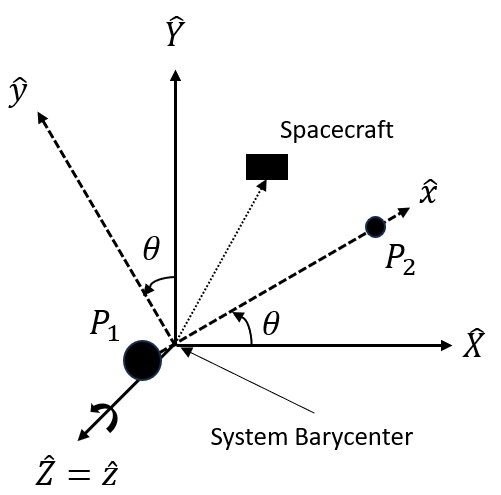
\includegraphics[width=0.5\textwidth]{figures/BaryFrames.jpg}
    \caption{Barycentric rotating and inertial frames in a CR3BP system.}
    \label{fig:baryFrames}
\end{figure}

\subsection{The Ecliptic J2000 Primary-Centered Inertial Frame}
A commonly used primary-centered inertial frame is the Ecliptic J2000. As the name implies, this
frame is established with its origin at the center of a primary body, and the Sun-Earth orbital
plane on January 1, 2000 as the $\Xhat_{Ec}\Yhat_{Ec}$-plane. The $\Xhat_{Ec}$-axis is directed
towards the vernal equinox, which is the line of intersection between the Earth's equatorial and
ecliptic planes on January 1, 2000. The $\Zhat_{Ec}$-axis is orthogonal to the ecliptic plane, and
the $\Yhat_{Ec}$-axis completes the triad, defined as $\Yhat_{Ec}=\Zhat_{Ec}\times\Xhat_{Ec}$.

Since the frame is centered on a primary, it is applicable to both the 2BP and CR3BP, making it
also valuable for patched dynamical models. The construction of this coordinate frame, as depicted
in \cref{fig:eclipJ2000Frame}, is computed using the Navigation and Ancillary Information
Facility's (NAIF) SPICE ephemeris toolkit\cite{Semenov:2023}.

\begin{figure}[ht]
    \centering
    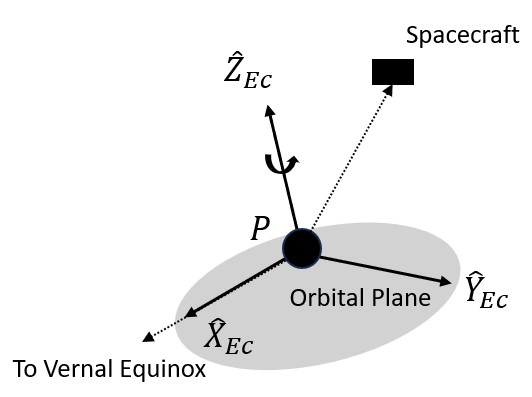
\includegraphics[width=0.5\textwidth]{figures/EclipJ2000Frame.jpg}
    \caption{Earth-centered Ecliptic J2000 inertial frame.}
    \label{fig:eclipJ2000Frame}
\end{figure}
